\documentclass{article}                          %%%定义文档类型
\usepackage[utf8]{inputenc}
\usepackage{ctex}                                %%%中文支持
\usepackage{amsmath}                             %%%数学公式包
\numberwithin{equation}{subsection}              %%%公式自动编号
\usepackage{geometry}
\geometry{left=0.95in,right=0.95in,top=1in,bottom=1in}
\usepackage{graphicx}                            %%%图片支持
\usepackage{caption}
\usepackage{float}
\usepackage[noblocks]{authblk}
\title{二维三角形单元上的高斯-勒让德数值积分公式}
%\author{李晓东$ ^{1} $\thanks{Email:lixiaodong112358@cug.edu.cn}\\$ ^{1} $中国地质大学(武汉)工程学院,地球深部能源实验室}
\author[*]{李晓东}
\affil[*]{中国地质大学(武汉)工程学院,地球深部能源实验室}
\begin{document}
	\maketitle
	\begin{abstract}
		本文给出了高斯积分公式在二维三角形区域的使用方法,首先给出了二维三角形单元的高斯-勒让德数值积分公式,而后给出了任意三角形单元的高斯数值积分公式,补充了足够的细节,并且给出了部分程序。
	\end{abstract}
\section{二维三角形参考单元上的高斯数值积分}
对于一个任意的三角形$ K $,总是可以通过仿射变换,将其映射到一个标准的三角形$ \hat{K} $,如图\ref{fig01}所示。因此我们首先需要解决在三角形参考单元$ \hat{K} $上的积分:
	\begin{figure}
		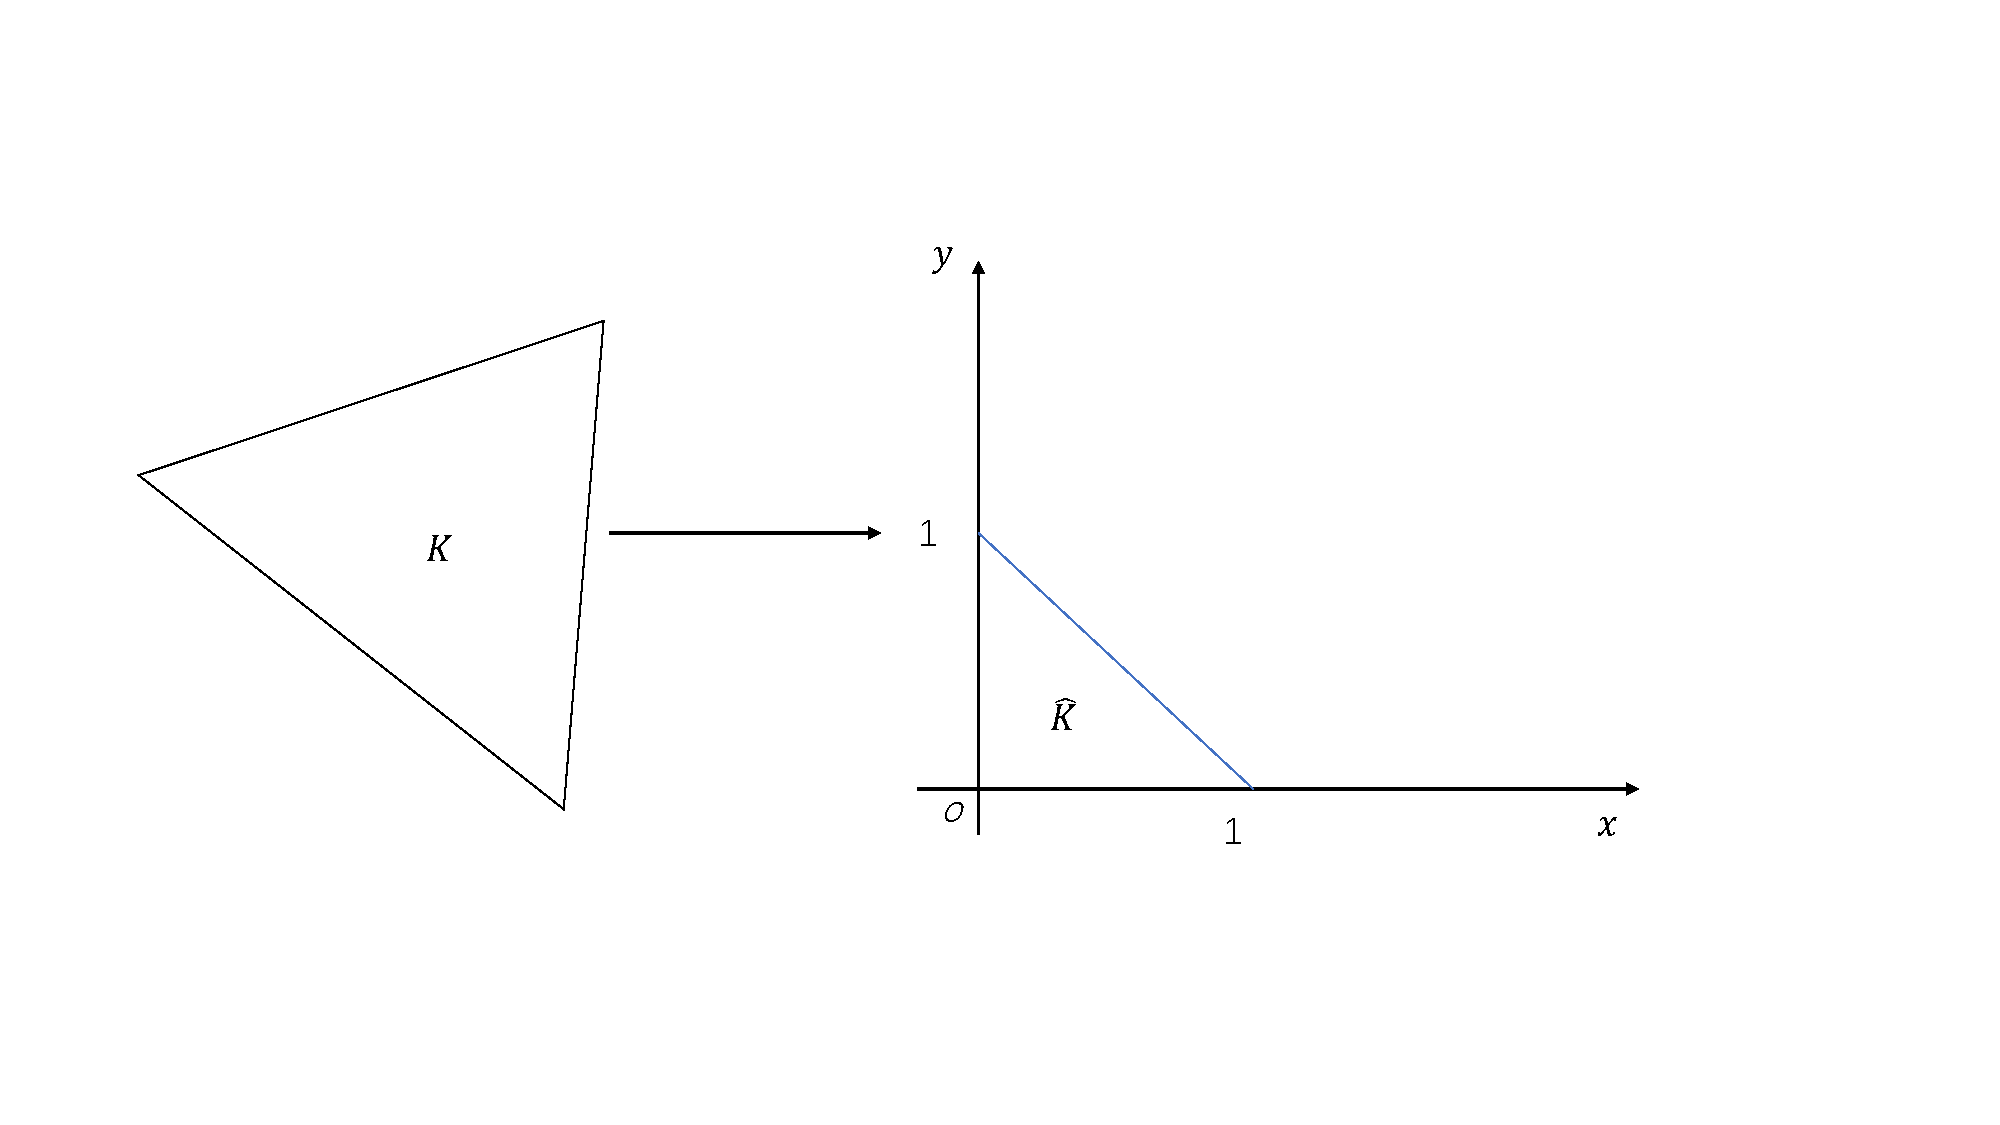
\includegraphics[width=\linewidth]{fig_triangle.pdf}
		\caption{任意三角形单元与三角形参考单元}
		\label{fig01}
	\end{figure}

	\begin{equation}\label{key}
	I=\iint_{\hat{K}}f(\hat{x},\hat{y})d\hat{x}d\hat{y}=\int_{0}^{1}d\hat{x} \int_{0}^{1-\hat{x}}f(\hat{x},\hat{y})d\hat{y}
	\end{equation}
做变量替换$ u=\hat{x},v=\frac{\hat{y}}{1-\hat{x}} $,则有$ 0\leq u,v \leq 1 $,那么有:
		\begin{equation}\label{key}
		\begin{aligned}
		\hat{x}&=u\\
		\hat{y}&=(1-u)v
		\end{aligned}
		\end{equation}
所以雅可比行列式$ J $为
		\begin{equation}\label{key}
		\frac{\partial (\hat{x},\hat{y})}{\partial (u,v)}=
		\begin{vmatrix}
		\frac{\partial \hat{x}}{\partial u}  &\frac{\partial \hat{x}}{\partial v} \\
		\frac{\partial \hat{y}}{\partial u}  &\frac{\partial \hat{y}}{\partial v}
		\end{vmatrix}
		=
		\begin{vmatrix}
		1   &0 \\
		-v  &1-u
		\end{vmatrix}=1-u
		\end{equation}
所以有:
		\begin{equation}\label{key}
		I=\int_{0}^{1} \int_{0}^{1} f(u,(1-u)v)(1-u)dudv
		\end{equation}
使用高斯积分,需要积分区间在$ [-1,1] $之间,因此需要做进一步的变换:
		\begin{equation}\label{key}
		u=\frac{1+\xi}{2},v=\frac{1+\eta}{2}
		\end{equation}
即:
		\begin{equation}\label{key}
		\xi=2u-1,\eta=2v-1
		\end{equation}
所以有:
		\begin{equation}\label{key}
		-1\leq \xi,\eta\leq 1, \frac{\partial (u,v)}{\partial (\xi,\eta)}=\frac{1}{4}
		\end{equation}
积分转化为:
		\begin{equation}\label{key}
		I=\int_{-1}^{1} \int_{-1}^{1} f(\frac{1+\xi}{2},\frac{(1-\xi)(1+\eta)}{4}) \frac{1-\xi}{8}d\xi d\eta
		\end{equation}
最后利用:
		\begin{equation}\label{key19}
		I=\sum_{i=1}^{n} \sum_{j=1}^{n}  f(\frac{1+\xi_i}{2},\frac{(1-\xi_i)(1+\eta_j)}{4}) \frac{1-\xi_{i}}{8} A_i A_j
		\end{equation}
式(\ref{key19})中 $ \xi_i $和$ \eta_j $ 为一维的高斯节点,$ A_i $和$ A_j$为一维的高斯权重,$ n $为高斯节点的数量,利用上式编程计算即可得到三角形参考单元的高斯积分值。

不过利用上式计算速度偏慢,因为每次计算都需要根据一维高斯节点生成相应三角形参考单元的高斯节点,事实上我们可以直接保存三角形参考单元的高斯节点和高斯权重,这样就不用那么麻烦了。\\
我们将式(\ref{key19})重新写为:
	\begin{equation}\label{key110}
	I=\sum_{k=1}^{N=n\times n}c_k f(x_k,y_k)
	\end{equation}
其中:
	\begin{equation}\label{key}
	c_k=\frac{1-\xi_i}{8} A_i A_j, x_k=\frac{1+\xi_i}{2},y_k=\frac{(1-\xi_i)(1+\eta_j)}{4},(k=1,\cdots,n^2),(i,j=1,\cdots,n)
	\end{equation}
	\begin{table}[H]
	\centering
	\caption{一维高斯节点和高斯权重}
	\label{table02}
	\begin{tabular}{lll}
\hline n & $ \xi_{i},\eta_j $ & $ A_{i} $ \\
\hline 1 & 0.0000000 & 2.0000000 \\
\hline 2 & $ \pm $ 0.5773503 & 1.0000000 \\
\hline & 0.7745967 & 0.5555556 \\
3 & 0.0000000 & 0.8888889 \\
\hline & $ \pm $ 0.8611363 & 0.3478548 \\
4 & $ \pm $ 0.3399810 & 0.6521452 \\
\hline & $ \pm $ 0.9061798 & 0.2369269 \\
5 & $ \pm $ 0.5384693 & 0.4786287 \\
& 0.0000000 & 0.5688889 \\
\hline & $ \pm $ 0.9324695 & 0.1713245 \\
6 & $ \pm $ 0.6612094 & 0.3607616 \\
& $ \pm $ 0.2386192 & 0.4679139 \\
\hline
\end{tabular}
\end{table}
	\begin{table}[H]
	\centering
	\caption{三角形参考单元的高斯节点和高斯权重}
	\label{table01}
	\begin{tabular}{lll}
	\hline $ x_{k} $ & $ y_{k} $ & $ c_{k} $ \\
	\hline n=2 & & \\
	0.211324865 & 0.166666667 & 0.197168783 \\
	0.211324865 & 0.622008467 & 0.197168783 \\
	0.788675134 & 0.044658198 & 0.052831216 \\
	0.788675134 & 0.166666667 & 0.052831216 \\
	n=3 & & \\
	0.112701665 & 0.100000000 & 0.068464377 \\
	0.112701665 & 0.443649167 & 0.109543004 \\
	0.112701665 & 0.787298334 & 0.068464377 \\
	0.500000000 & 0.056350832 & 0.061728395 \\
	0.500000000 & 0.250000000 & 0.098765432 \\
	0.500000000 & 0.443649167 & 0.061728395 \\
	0.887298334 & 0.012701665 & 0.008696116 \\
	0.887298334 & 0.056350832 & 0.013913785 \\
	0.887298334 & 0.100000000 & 0.008696116 \\
	\hline
\end{tabular}
\end{table}

其中一维高斯节点与高斯权重如表\ref{table02}所示,部分三角形参考单元的高斯节点和高斯权重值如表\ref{table01}所示,本人在附录中给出了示例MATLAB程序,读者可以自行参考。


\section{任意三角形单元上的高斯数值积分}
在微积分理论中,有二重积分的换元公式:
\begin{equation}\label{key201}
\iint_K f(x,y)dxdy=\iint_{\hat{K}} f(x(\hat{x},\hat{y}),y(\hat{x},\hat{y}))|J|d\hat{x}d\hat{y}
\end{equation}
从任意三角形单元$ K $到三角形参考单元$ \hat{K} $的仿射变换为:
	\begin{equation}\label{key}
	\begin{aligned}
	\left(\begin{array}{l}
	x \\
	y
	\end{array}\right) &=\left(A_{2}-A_{1}, A_{3}-A_{1}\right)\left(\begin{array}{l}
	\hat{x} \\
	\hat{y}
	\end{array}\right)+A_{1} \\
	&=\left(\begin{array}{ll}
	x_{2}-x_{1} & x_{3}-x_{1} \\
	y_{2}-y_{1} & y_{3}-y_{1}
	\end{array}\right)\left(\begin{array}{l}
	\hat{x} \\
	\hat{y}
	\end{array}\right)+\left(\begin{array}{l}
	x_{1} \\
	y_{1}
	\end{array}\right)
	\end{aligned}
	\end{equation}
	其中$ x_1,x_2,x_3,y_1,y_2,y_3$分别为三角形三个顶点的坐标。
	\begin{equation}\label{key}
	\begin{aligned}
	\hat{x} &=\frac{\left(y_{3}-y_{1}\right)\left(x-x_{1}\right)-\left(x_{3}-x_{1}\right)\left(y-y_{1}\right)}{|J|} \\
	\hat{y} &=\frac{-\left(y_{2}-y_{1}\right)\left(x-x_{1}\right)+\left(x_{2}-x_{1}\right)\left(y-y_{1}\right)}{|J|}
	\end{aligned}
	\end{equation}
	雅可比矩阵绝对值$ |J| $为:
	\begin{equation}\label{key}
	|J|=|\left(x_{2}-x_{1}\right)\left(y_{3}-y_{1}\right)-\left(x_{3}-x_{1}\right)\left(y_{2}-y_{1}\right)|
	\end{equation}	
结合式\ref{key110}与式\ref{key201}可以得到:
\begin{equation}\label{key}
I=\sum_{k=1}^{N=n\times n}c_k f(x(x_k,y_k),y(x_k,y_k))|J|
\end{equation}
根据上式编程求解,即可计算任意三角形单元的数值积分。
\section{参考文献}
[1] Rathod H T ,  Nagaraja K V . Gauss Legendre Quadrature over a Triangle[J]. Journal of the Indian Institute of Science, 2004.
\section{附录}

		\begin{verbatim}
	function result=generate_Gauss_reference_2D_triangle(Gauss_type)
	%%%%根据一维高斯节点和高斯权重,生成三角形参考单元的高斯节点高斯权重
	%%%%2021/5/8,李晓东
	[Gauss_weight,Gauss_nodes]=generate_Gauss_reference_1D(Gauss_type);
	vector=zeros(Gauss_type*Gauss_type,3);
	k=1;
	for i=1:Gauss_type
	for j=1:Gauss_type
	vector(k,1)=(1+Gauss_nodes(j))/2;
	vector(k,2)=(1-Gauss_nodes(j))*(1+Gauss_nodes(i))/4;
	vector(k,3)=(1-Gauss_nodes(j))/8*Gauss_weight(j)*Gauss_weight(i);
	k=k+1;
	end
	end
	result=vector;
	end
	\end{verbatim}
	\begin{verbatim}
	function [Gauss_weight,Gauss_nodes]=generate_Gauss_reference_1D(Gauss_type)
	%%根据高斯节点数目,返回相应的高斯节点与高斯权重系数
	if Gauss_type==4
	Ai=[0.3478548451,0.3478548451,0.6521451549,0.6521451549];
	xi=[0.8611363116,-0.8611363116,0.3399810436,-0.3399810436];
	elseif Gauss_type==8
	Ai=[0.1012285363,0.1012285363,0.2223810345,0.2223810345,...
	0.3137066459,0.3137066459,0.3626837834,0.3626837834];
	xi=[0.9602898565,-0.9602898565,0.7966664774,-0.7966664774,...
	0.5255324099,-0.5255324099,0.1834346425,-0.1834346425];
	elseif Gauss_type==2
	Ai=[1,1];
	xi=[-1/sqrt(3),1/sqrt(3)];
	elseif Gauss_type==3
	Ai=[0.555555556,0.555555556,0.88888889];
	xi=[0.7745966692, -0.7745966692,  0];
	else
	warning='高斯点数请在2、3、4、8中选取'
	end
	Gauss_weight=Ai;
	Gauss_nodes=xi;
	end
	\end{verbatim}

\end{document}